% Finite-depth teacher diagnostics only; not route quality or PPO performance.
\begin{figure*}[t]
\centering
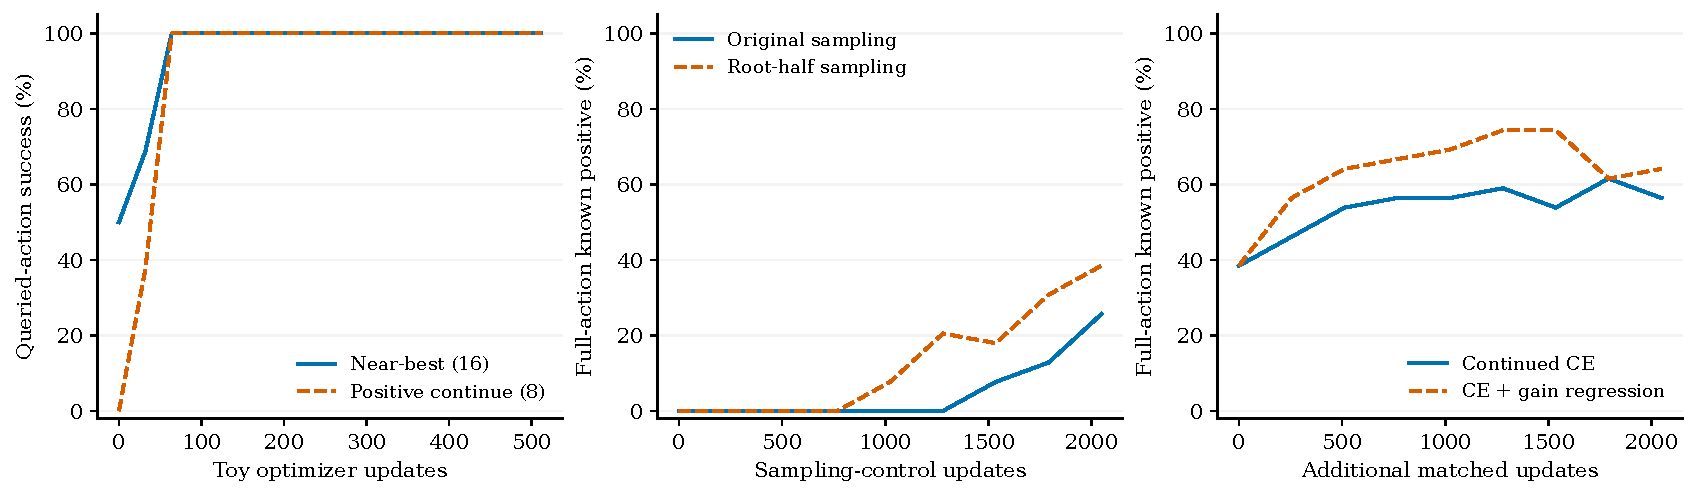
\includegraphics[width=0.95\textwidth]{figures/training_curves.pdf}
\caption{Bounded offline diagnostics, one seed and no new environment queries. Left: fitting 16 selected training roots within queried actions. Middle: original versus root-half sampling, each 2,048 updates from the same frozen BC. Right: another matched 2,048 updates from the final root-half checkpoint, comparing CE and CE plus root-depth-2 gain regression. The middle and right panels measure full-legal-action selection of a known positive action on the same 39 positive training roots. Intermediates are diagnostic only; every gate uses the prescribed final update.}
\label{fig:g21_training}
\end{figure*}
\begin{figure*}[t]
\centering
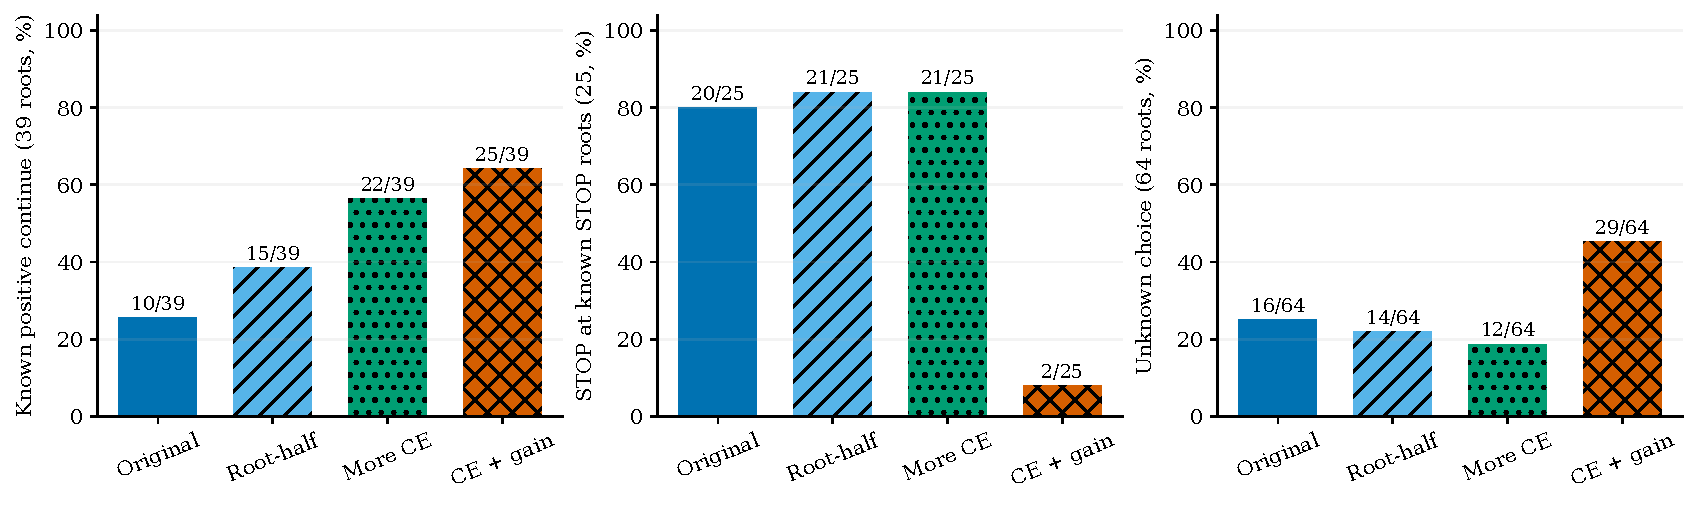
\includegraphics[width=0.95\textwidth]{figures/final_diagnostics.pdf}
\caption{Single-seed final-checkpoint full-action diagnostics on the original 64 training roots. Gain supervision improves known-positive detection relative to its matched continued-CE control, but has fewer STOP selections at roots where STOP is best among queried actions, and selects more unknown actions. Unknown actions have not been evaluated and are not classified as poor actions. Original/root-half have 2,048 additional updates; More CE/CE+gain have 4,096 additional updates in their respective lineages. Only the paired comparisons isolate sampling or the auxiliary objective. These are finite-teacher diagnostics, not new-scene planning benefits.}
\label{fig:g21_final}
\end{figure*}
